\begin{chapter}{\label{cha:numerics}Numerical Algorithms}
\section{\label{section:RK} Numerical procedures for 2D and 3D solutions}
	\subsection{\label{section:RK4} Fourth order Runge-Kutta scheme}
	The classical fourth-order Runge-Kutta formula (RK4) is described equivalently in many texts. We follow the description in \cite{NumericalRecipes}. Let an initial value problem be specified as
	
	\begin{align*}
		\frac{\partial \psi}{\partial t} &= f(\psi,t),\hspace{0.25in}\psi(t_0) = \psi_0.
	\end{align*}

A step-size, $h>0$, is chosen as the parameter controlling how the solution is advanced over $t$. The scheme for estimating $\psi(t_n)= \psi_n$ is then written
\begin{equation}
\begin{split}
		k_1 &= hf(t_n,\psi_n),\\
		k_2 &= hf(t_n+\frac{h}{2},\psi_n+\frac{k_1}{2}),\\
		k_3 &= hf(t_n+\frac{h}{2},\psi_n+\frac{k_2}{2}),\\
		k_4 &= hf(t_n+h,\psi_n+k_3),\\
		\psi_{n+1} &= \psi_n + \frac{k_1}{6}+ \frac{k_2}{3}+ \frac{k_3}{3} + \frac{k_4}{6} + \mathcal{O}(h^5),\\
		t_{n+1}  &= t_n + h.
		\label{eq:rk4}
\end{split}
\end{equation}


	An outline derivation of the Runge-Kutta scheme, which includes a proof of accuracy are shown in Appendix \ref{appsection:rk4deriv}.
	In all of our relevant calculations the value of f is set as the right hand side of the homogeneous or trapped GPE. The main loop formulating the RK4 method may be repeated indefinitely to reach any $t>t_0$. The step size for a given set of parameters should be chosen small enough that smaller choices make no quantitative changes to the resulting solution. The following section outlines the methods we have implemented to ensure numerical solutions are converged.

	\subsection{\label{section:numericalParams} Numerical stability and convergence}
	We now investigate numerical parameters which affect the stability of simulated superfluid systems. Our direct aim is to find a suitable discretisaton of space and time so that while simulations are timely, our numerical quantities are converged (so that they are not sensitive to small changes in computational parameters) and that quantities conserved by the equations of motion are indeed conserved in the computed numerical solutions.

	We begin by estimating $\Delta_x$, the required spacial grid spacing, by considering the width of the vortex core in a homogeneous system, a feature we would like well and accurately visualised in our numerical solutions. Through observation of a singly quantised vortex core (as in Figure \ref{fig_vortex}) we observe a core radius of approximately $5\xi$ when the background density is $\rho=1$. To ensure the vortex core structure is well resolved we decide to dedicate 10 grid points for a vortex core radius, suggesting a value of $\Delta_x = \xi/2$.

	In the trapped case we can use the same idea. It is shown in Section \ref{section:healing} that $\xi = \hbar/\sqrt{mg}$ for $\rho=1$. We can then easily rearrange to find an expression for $\xi$ in the harmonic oscillator units of trapped condensates. We find that our approximate grid spacing to adequately resolve the vortex core is $\Delta_x = 0.5\xi = 0.5\omega \sqrt{\hbar/(\mu \omega)} l_r$. As an example, for a trapped condensate with interaction energy $\hat{g}=2000$, chemical potential $\hat{\mu}=25.27$ and trap frequency $\omega=8.75~{\rm Hz}$ we find that a value of $\Delta_x=0.1l_r$ should be adequate. 

	Similar arguments (concerned with time rather than space), can be used to approximate a suitable time step $h$. We define a time period that we would like to be well resolved by considering by the smallest possible element moving at the fastest reasonable speed. If we define this period as $\Delta_x / 5~c$ and allocate to it 10 time steps, we find that $h = 0.5\xi/50~c = 0.01\tau$.

  In addition to this process, for each set of simulation parameters it is recommended to confirm the suitability of the chosen $\Delta_x$ and $h$ by testing the convergence and conservation in the numerical methods. The total condensate energy and particle number are good measures for this as they should both be well conserved by the GPE with a dissipation of $\gamma=0$. An example of this process (confirming the suitability of a chosen $\Delta_x$) is shown in Figure \ref{fig_energ_norm_cons}: For a large $\Delta_x=0.4l_r$ both the condensate energy and norm fluctuate wildly. For $\Delta_x=0.1l_r$ the norm is extremely well conserved to within $2.10^{-5}\%$ and the energy is conserved within $5.10^{-3}\%$. The smallest tested value of $\Delta_x=0.05l_r$ finally confirms that the energy has converged. We conclude that for the chosen system parameters that $\Delta_x=0.1l_r$ (the value suggested by the above analysis) is numerically sufficient and there is little reason to use $\Delta_x<0.1l_r$.

  \begin{figure}
  \centering
   \begin{tikzpicture}
    \begin{axis}[y tick label style={
            /pgf/number format/.cd,
                fixed,
                fixed zerofill,
                precision=3,
            /tikz/.cd
        },
        width=0.98\linewidth,
        height=0.3\linewidth,
        xlabel={},
        ylabel=$\hat{E}\left ( \hat{t} \right )$,
        xmin=0,
        xmax=10,
        major tick length = 0.07cm
      ]
      \addplot gnuplot [raw gnuplot,mark=none,color=black,thick]{
        plot "numerics/figures/energ-norm-cons.0.05" using 1:3 with lines;
      };
      \addplot gnuplot [raw gnuplot,mark=none,color=red,thick]{
        plot "numerics/figures/energ-norm-cons.0.1" using 1:3 with lines;
      };
      \addplot gnuplot [raw gnuplot,mark=none,color=green,thick]{
        plot "numerics/figures/energ-norm-cons.0.2" using 1:3 with lines;
      };
      \addplot gnuplot [raw gnuplot,mark=none,color=blue,thick]{
        plot "numerics/figures/energ-norm-cons.0.4" using 1:3 with lines;
      };
    \end{axis}
  \end{tikzpicture}
  \begin{tikzpicture}
    \begin{axis}[y tick label style={
            /pgf/number format/.cd,
                fixed,
                fixed zerofill,
                precision=4,
            /tikz/.cd
        },
        width=0.98\linewidth,
        height=0.35\linewidth,
        name=mainplot,
        xlabel=$\hat{t}$,
        ylabel=$\hat{N}\left ( \hat{t} \right )$,
        xmin=0,
        xmax=10,
        ymax=1.0008,
        major tick length = 0.07cm
      ]
      \addplot gnuplot [raw gnuplot,mark=none,color=black,thick]{
        plot "numerics/figures/energ-norm-cons.0.05" using 1:4 with lines;
      };
      \addplot gnuplot [raw gnuplot,mark=none,color=red,thick]{
        plot "numerics/figures/energ-norm-cons.0.1" using 1:4 with lines;
      };
      \addplot gnuplot [raw gnuplot,mark=none,color=green,thick]{
        plot "numerics/figures/energ-norm-cons.0.2" using 1:4 with lines;
      };
      \addplot gnuplot [raw gnuplot,mark=none,color=blue,thick]{
        plot "numerics/figures/energ-norm-cons.0.4" using 1:4 with lines;
      };
      \node[anchor=west] (source) at (axis cs:9.25,1.00027){};
      \node[anchor=west] (destination) at (axis cs:9.25,1.0000){};
      \node[anchor=west] (topl) at (axis cs:9.2,1.00005){};
      \node[anchor=west] (botr) at (axis cs:9.8,0.99995){};
      \draw[->](source)--(destination);
      \draw(topl) rectangle (botr);
    \end{axis}
    \begin{axis}[y tick label style={
            /pgf/number format/.cd,
                fixed,
                fixed zerofill,
                precision=6,
            /tikz/.cd
        },
        width=0.35\linewidth,
        height=0.18\linewidth,
        at={(mainplot.north east)},anchor=north east,
        xlabel={},
        ylabel={},
        xmin=9.15,
        xmax=9.85,
        major tick length = 0.07cm
      ]
      \addplot gnuplot [raw gnuplot,mark=none,color=black,thick]{
        plot "numerics/figures/energ-norm-cons.0.05" using 1:4 with lines;
      };
      \addplot gnuplot [raw gnuplot,mark=none,color=red,thick]{
        plot "numerics/figures/energ-norm-cons.0.1" using 1:4 with lines;
      };
      \addplot gnuplot [raw gnuplot,mark=none,color=green,thick]{
        plot "numerics/figures/energ-norm-cons.0.2" using 1:4 with lines;
      };
    \end{axis}
  \end{tikzpicture}
  \caption{Dimensionless energy, $\hat{E}$, and particle number, $\hat{N}$, throughout numerical propagation of a trapped condensate containing a singly quantised vortex in its center, with interaction energy $\hat{g}=2000$ and chemical potential $\hat{\mu}=25.27$. The numerical grid width varies with each line; (black) $\Delta_x = 0.05$, (red) $\Delta_x = 0.1$, (green) $\Delta_x = 0.2$ and (blue) $\Delta_x = 0.4$. (Inset) Zoomed view of the convergence of $\hat{N}$.}\label{fig_energ_norm_cons}
 \end{figure}

\section{\label{section:vortexidentifying} Identifying vortices}
Large potions of this thesis are dedicated to the study of 2D vortex dynamics. As such, accurate detection of the location and charge of densely packed quantised vortices is required, and so we have developed robust numerical methods for vortex identification. The basic idea is fairly simple, with arguments similar to those used in Section \ref{section:quantisedcirculation} to demonstrate the quantised nature of the circulation.

The integrated change of phase along any closed curve $C$ is,
\begin{equation}
  \Delta\theta(C) = \oint_C \! \nabla \theta  \, \mathrm{d}\mathbf{l} = 2\pi q,
\end{equation}
where $\mathrm{d}\mathbf{l}$ is the line element and $q\in\mathbb{Z}$. Further, the fundamental theorem of calculus for line integrals[CITE] implies that $\Delta\theta(C) = 0$, providing that $C$ is continuous and does not encompass a phase singularity. This result is crucial, as it allows us to directly state that a vortex lies within $C$ if and only if $|\Delta\theta(C)| > 0 $.

\subsection{\label{section:vortexloc} Basic vortex detection method}
First define a set of curves $C_k$ with each curve lying on points of our numerical grid, so that a single $C_k$ encompasses only a small region of the fluid (ideally, $C_k$ should encompass a region at most the diameter of a vortex core). $\Delta\theta(C_k)$ is then approximated for each $k$ using numerical integration. If $\Delta\theta(C_k) = 0$ (to within numerical accuracy) then we say the region inside $C_k$ contains no vortices. Otherwise the sign of $\Delta\theta(C_k)$ tells us the polarity of the vortex.

In principle the result also allows us to calculate the exact charge of a vortex in terms of the quantum of circulation. However, for accurate determination of vortex location, the curves $C_k$ must encompass a very small area. In some cases the numerical integration uses only on the order of $10$ grid points and so integration accuracy is low. Nevertheless, using only the sign of the $\Delta\theta(C_k)$ results in an accurate detection of vortex polarity and location and as multiply charged vortices are unstable (rapidly decaying into several singly charged vortices) there is no significant loss.
\begin{figure}
  \centering
   \begin{tikzpicture}[
        >={Straight Barb[left]},
      myarrow/.style={
        decoration={
          markings,
          mark=at position 0.5 with {\arrow{Straight Barb[left]}};
          },
        postaction=decorate  
        }
      ]
      \begin{axis}[
        xlabel={Numerical grid (x)},
        ylabel={Numerical grid (y)},
        xtick={0,10,20,30,40,50},
        ytick={0,10,20,30,40,50},
        x=1cm/10,
        y=1cm/10,
        xmin=0,
        xmax=50,
        ymin=0,
        ymax=50,
        colorbar style={title={Phase},text width=0.5em,major tick length = 0.07cm},
        major tick length = 0.07cm,
        point meta min = -3.1415,
        point meta max = 3.1415,
        colorbar,colormap name=hsvcl
      ]
      \addplot graphics [xmin=0,xmax=50,ymin=0,ymax=50] {numerics/figures/vortex1dp-hsv.png};
    \end{axis}
      \draw[step=1cm,gray,very thin] (0,0) grid (5,5);
      \foreach \i in {1,...,5}{
        \foreach \j in {1,...,5}{
          \draw [myarrow,thick] (\i-0.05,5.95-\j)--(\i-0.95,5.95-\j);
          \draw [myarrow,thick] (\i-0.95,5.95-\j)--(\i-0.95,5.05-\j);
          \draw [myarrow,thick] (\i-0.95,5.05-\j)--(\i-0.05,5.05-\j);
          \draw [myarrow,thick] (\i-0.05,5.05-\j)--(\i-0.05,5.95-\j);
          {\pgfmathtruncatemacro{\label}{((\j-1)*5) + \i}
          \node[] (c0) at (\i-0.5,5.5-\j) {$C_{\label}$};}
        }
      }
  \end{tikzpicture}
  \caption{Example of a set of curves $C_k$ for identifying a vortex (located at [12.5,12.5]). All $\Delta\theta(C_{k\neq13})\approx0$, and $\Delta\theta(C_{13})>0$. The conclusion is that a positive vortex lies in the region defined by $C_{13}$.}
 \end{figure}
\subsection{\label{section:vortexloc} Visualising vortex location with a vortex field}
The basic vortex identification method set out in \ref{section:vortexloc} is quick to implement and useful when there are few well separated vortices, but one can easily imagine a situation where the system fails. One such case would be two vortices both lying within a single $C_k$ curve; only a single vortex would be detected.

The solution is not always as simple as reducing the size of $C_k$, there are often too little grid points to make this reasonable. Instead curves with a size remaining around the size of a vortex core are used, but for every grid point (taking into account boundary conditions) in the simulation the curve $C_{i,j}$ is defined surrounding and centred on the pixel [i,j]. A vortex field can then be visualised by viewing the 2D plot of $\Delta\theta(C_{i,j})$. Sub pixel accuracy can then be found by averaging the location of all points where $|\Delta\theta(C_{i,j})|>\Delta_t$, where $\Delta_t$ is some threshold value.
%for i=1:50
%for j=1:50
%test(i,j)=atan2(j-25.5,i-23)-atan2(j-25.5,i-27);
%end
%end
\subsection{\label{section:gaussianblur} Further improve accuracy with a Gaussian blur}
\subsection{\label{section:ghostvortex} Avoiding `ghost vortices'}


\section{\label{section:vortexclustering} Quantifying vortex clustering}
	\subsection{\label{section:reevesalgorithm} Recursive Cluster Algorithm (RCA) }
		


	\subsection{\label{section:ripleysk} Ripley's K function }
		\begin{equation}\label{eq:ripleysk}
		K(x) = \frac{A}{n^2}\sum\limits_{i \ne j} I\left (d_{ij}<x\right ),
		\end{equation}
		where $d_{ij}$ is the distance between the $i$th and $j$th points, $A$ is the area of the region containing every point, $n$ is the number of points, $x$ is the search radius, and I is the indicator function (1 if its argument is true, 0 otherwise). Should the points be distributed homogeneously in space, then $K(s)\approx\pi s^2$.
\section{\label{section:vortextracking} Tracking vortex trajectories}
\section{\label{section:vortexremoval} Removing vortices with phase unwrapping}

\section{\label{section:quasi-condensate} Quasi-Condensate Visualisation}
When in the context of the classical-field method of simulating a finite temperature Bose gas, the raw numerical wavefunction is too noisy to allow direct visualization of vortical structures, this can be overcome by defining a quasi-condensate wavefunction $\hat{\psi}$, as established in \cite{PhysRevA.66.013603}.   This wavefunction is constructed by filtering out high-frequency spatial modes from the classical field wavefunction, by 
transforming the complex amplitudes via
$\hat{a}_{{\bf k}} = a_{{\bf k}}\times\max\{1-k^{2}/k_c^2,0\}$. $\hat{\psi}$ represents the long-wavelength component of the classical field.

The choice of $k_c$ is facilitated by the the bimodal distribution of occupation numbers in the wavefunction, a distribution which develops naturally through propagation of the GPE. The high-$k$ part of the distribution is associated with the thermal excitations and low mode occupations. The low-$k$ part of the field is the quasi-condensate, characterised by macroscopic mode populations and superfluid ordering. $k_c$ is chosen as the boundary in $k$-space between the quasi-condensate and the thermal gas, as performed in \cite{PhysRevA.66.013603}. Figure \ref{fig:quasicondensatefilter} demonstrates the filtering technique in action.
\begin{figure}
\centering
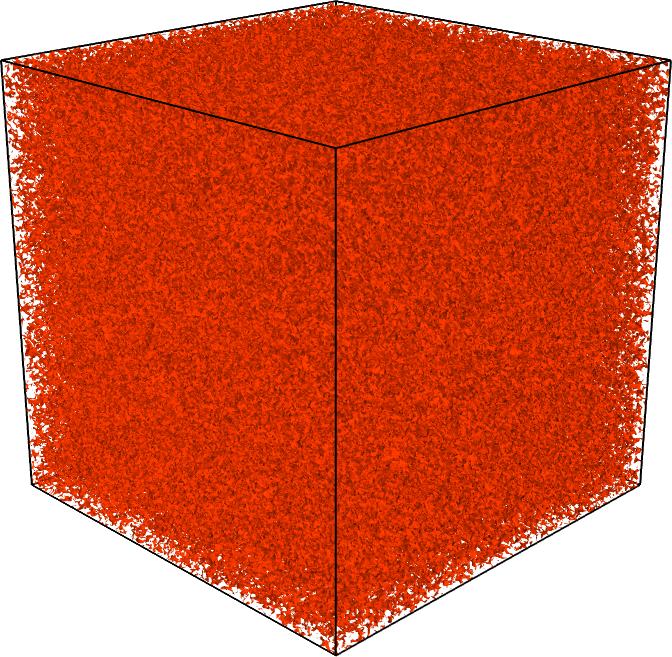
\includegraphics[width=0.4\linewidth]{numerics/figures/mess3d}%
    \begin{minipage}[b]{0.2\linewidth}
      \centering
      \raisebox{3cm}{$\longrightarrow$}
    \end{minipage}% 
    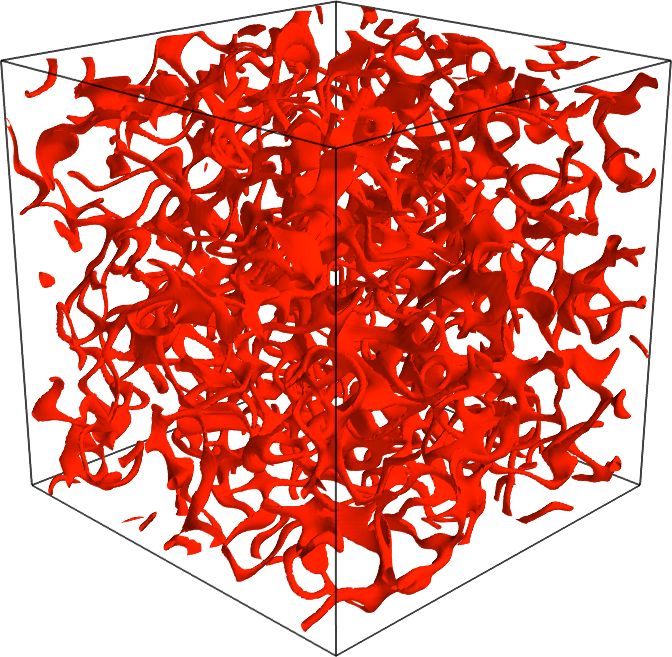
\includegraphics[width=0.4\linewidth]{numerics/figures/clean3d}
  \caption{(Left) Unfiltered wavefunction density, $|\psi|^2$, from a classical-field simulation with condensate fraction $\rho_0/\rho=0.22$ during equilibration. A vortex tangle is present but not visible by direct density visualisation. (Right) Filtered wavefunction density, $|\hat{\psi}|^2$, clearly showing the vortical structures in the gas.}\label{fig:quasicondensatefilter}
  \end{figure}
  	
\section{\label{section:linelength} Evaluation of vortex line-length}
For a given wavefunction, $\Psi$, featuring a vortex distribution, the vortex volume $V_t$ (the total volume associated with the vortex cores) is evaluated by numerical integration of the inside of the vortex isosurface tubes obtained from the filtered density $|\hat \Psi|^2$, with an integration region of the whole numerical box.  Note that the isosurface level should be low enough to pick out vortex cores only (and not, e.g. fluctuations and waves), while large enough to contain sufficient grid points to allow a reasonable numerical evaluation of volume. In this work we use the isosurface level $0.04\langle |\hat{\Psi}|^2 \rangle$ (chosen so as to produce filtered vortex cores that are similar in radius to the true vortex core).  The volume calculation can be written $V_t = \int \Theta(0.04\langle |\hat{\Psi}|^2 \rangle - |\hat{\Psi}({\bf r})|^2)~{\rm d}V$, where $\Theta$ is the Heaviside step function. In practice the calculation of the vortex core volume can be efficiently performed by assigning a value of unity/zero to grid points located within/outside the isosurface tubes and directly integrating the result using the trapezium or Simpson's rule.

The total line length is then deduced by dividing $V_t$ by the cross-sectional area of a vortex core, $A_t$ (in effect, the average cross-sectional area of the isosurface tubes). The measured values of $V_t$ and $A_t$ will depend on the chosen isosurface level but, providing the vortex tubes are well-separated, their ratio (and hence the evaluated line length) will remain constant.  For closely-positioned vortex tubes, the isosurface level can affect whether the tubes appear as two separate tubes, or start to merge, and so will lead to deviations in this ratio.  We have tested the effect of an alternative isosurface value.  For twice the original isosurface value, the difference in the calculated line length is negligible for systems with low vortex density.  For cases with the highest density of vortices, the difference remains less than $10\%$.

\end{chapter}
